% 第五章：留数理论

\chapter{留数理论}

\begin{wulibj}[本章导读]
上一章最后，我们已经看到一个很关键的事实：在奇点附近作洛朗展开时，负幂项记录的是奇点的异常结构；而当我们沿着包围奇点的小圆做积分时，别的幂次项几乎都会被``筛掉''，只有
\[
    \frac{c_{-1}}{z-z_0}
\]
这一项会真正留下来。本章要做的，就是把这条观察正式提升为留数概念，并进一步说明：为什么一个看起来只属于\textbf{局部展开}的系数，居然能够控制\textbf{整体闭路积分}，甚至帮助我们计算实积分、研究零点和极点的个数。

从主线看，本章可以概括为：
\[
    \text{洛朗展开中的 } c_{-1}
    \Longrightarrow
    \text{留数}
    \Longrightarrow
    \text{留数定理}
    \Longrightarrow
    \text{积分计算与零点计数}.
\]
\end{wulibj}

\begin{wulibj}[物理背景]
留数理论之所以重要，不只是因为它在数学上漂亮，更因为它在物理问题中真的有用。

\textbf{1. 振动与波动：}在研究受迫振动、频域响应和波包传播时，经常会遇到含极点的复函数。极点的位置往往反映系统的特征频率，而留数则刻画该模态贡献的强弱。

\textbf{2. 量子力学：}散射理论与格林函数方法中，极点结构常和束缚态、共振态联系在一起；相应留数又和这些态的权重密切相关。

\textbf{3. 流体力学与保角映射：}在二维势流问题里，复势函数的奇点和留数常常有直接物理解释，例如点源、点涡和升力公式等。

\textbf{4. 积分变换：}傅里叶变换、拉普拉斯变换的逆变换，很多时候都会归结为复平面上的围道积分，而留数定理正是最核心的计算工具之一。
\end{wulibj}

\begin{tishi}[先把本章主线抓住]
这一章最重要的，不是记住几条求留数公式，而是建立下面这个认识：\textbf{留数是奇点附近最能影响积分的局部信息。}一旦这件事想清楚，后面的留数定理、单位圆方法、半圆围道方法、辐角原理都会显得顺理成章。
\end{tishi}

\section{从局部展开到留数}

\begin{wulibj}[本节的任务]
这一节不是为了引入很多新计算，而是为了把上一章末尾已经看到的现象收束成一个明确概念：为什么一阶负幂项最特殊，为什么它值得单独命名，以及它到底在记录奇点附近的什么信息。
\end{wulibj}

上一章已经证明：若函数在某个孤立奇点附近能作洛朗展开，那么围绕该奇点的小圆积分对绝大多数幂次项都不敏感。现在我们把这个结论重新压缩成一条本章的起点结论。

\subsection{为什么一阶负幂项最特殊}

设 $z_0$ 是 $f$ 的孤立奇点，$C_\rho$ 是绕 $z_0$ 的正向小圆：
\[
    z-z_0=\rho\mathrm{e}^{\mathrm{i}\theta},\qquad 0\le \theta\le 2\pi.
\]
若在该小圆附近有洛朗展开
\[
    f(z)=\sum_{n=-\infty}^{\infty} c_n (z-z_0)^n,
\]
那么围道积分会发生一种非常鲜明的``筛选''现象。

\begin{tuilun}{小圆积分只认一阶负幂项}{}
若 $f$ 在小圆 $C_\rho$ 上可写成
\[
    f(z)=\sum_{n=-\infty}^{\infty} c_n (z-z_0)^n,
\]
则
\[
    \oint_{C_\rho} f(z)\,\mathrm{d}z
    =
    2\pi \mathrm{i}\, c_{-1}.
\]
\end{tuilun}

\begin{proof}
由上一章已经证明过的结论，洛朗级数在较小闭圆环上一致收敛，因此在小圆 $C_\rho$ 上可以逐项积分：
\[
    \oint_{C_\rho} f(z)\,\mathrm{d}z
    =
    \sum_{n=-\infty}^{\infty} c_n
    \oint_{C_\rho} (z-z_0)^n\,\mathrm{d}z.
\]
而对整数 $n$，上一章还已经证明
\[
    \oint_{C_\rho}(z-z_0)^n\,\mathrm{d}z
    =
    \begin{cases}
        0, & n\ne -1,\\[4pt]
        2\pi \mathrm{i}, & n=-1.
    \end{cases}
\]
所以所有项都被筛掉，只有 $n=-1$ 这一项留下来，故
\[
    \oint_{C_\rho} f(z)\,\mathrm{d}z
    =
    2\pi \mathrm{i}\, c_{-1}.
\]
\end{proof}

\begin{figure}[htbp]
\centering
\begin{tikzpicture}[scale=0.95]
    \draw[->, gray] (-3.1,0) -- (3.4,0) node[right] {$\operatorname{Re} z$};
    \draw[->, gray] (0,-2.8) -- (0,3.1) node[above] {$\operatorname{Im} z$};

    \fill[red] (0,0) circle (2.4pt);
    \node[below left] at (0,0) {$z_0$};

    \draw[blue, thick, ->] (2,0) arc[start angle=0,end angle=330,radius=2];
    \node[blue] at (2.35,1.35) {$C_\rho$};

    \node[align=center] at (-1.9,1.7) {$\dfrac{c_{-2}}{(z-z_0)^2}$\\积分后消失};
    \node[align=center, text=importantred] at (0,2.3) {$\dfrac{c_{-1}}{z-z_0}$\\被保留下来};
    \node[align=center] at (1.95,1.7) {$c_0,\ c_1(z-z_0),\dots$\\积分后消失};

    \draw[gray, dashed] (-1.85,1.2) -- (-0.95,0.8);
    \draw[importantred, dashed] (0,1.95) -- (0,1.05);
    \draw[gray, dashed] (1.85,1.2) -- (0.95,0.8);

    \node at (0,-2.05) {$\displaystyle \oint_{C_\rho} f(z)\,\mathrm{d}z = 2\pi \mathrm{i}\, c_{-1}$};
\end{tikzpicture}
\caption{小圆积分的筛选机制：只有一阶负幂项会留下来}
\label{fig:residue-local-contour}
\end{figure}

\begin{zhu}{}{}
这一条结论非常值得反复咀嚼。它说明围道积分并不是把奇点附近的所有细节一视同仁地都看一遍，而是在许多局部信息里只抓住最关键的那一项。下一步要做的，就是把这个特殊系数单独命名。
\end{zhu}

\subsection{留数的定义}

\begin{dingliyi}{留数}{}
设 $z_0$ 是 $f(z)$ 的孤立奇点，且在 $z_0$ 的某个穿孔邻域内有洛朗展开
\[
    f(z)=\sum_{n=-\infty}^{\infty} c_n (z-z_0)^n.
\]
称系数 $c_{-1}$ 为 $f(z)$ 在 $z_0$ 处的\textbf{留数}，记作
\[
    \operatorname{Res}[f(z),z_0]=c_{-1}.
\]
\end{dingliyi}

\begin{tishi}[这一定义为什么自然]
因为对小圆积分来说，真正会留下贡献的正是 $c_{-1}$。也就是说，留数不是凭空规定出来的记号，而是被围道积分``选中''的那个局部系数。
\end{tishi}

\subsection{留数到底在记录什么}

从形式上看，留数只是洛朗展开中的一个系数；但从意义上看，它记录的是\textbf{奇点附近对围道积分最敏感的那部分局部信息}。这句话里有两层意思：

\begin{enumerate}
    \item 留数并不是奇点的全部信息。例如二阶极点、本性奇点、可去奇点，它们的整体结构差别很大，单看留数并不能完全区分。
    \item 但在积分问题里，留数又往往已经够用了。因为围道积分只留下这一项，所以很多整体积分最终真的只需要求若干个留数。
\end{enumerate}

\begin{lizi}{由洛朗展开直接读取留数}{}
求
\[
    f(z)=\frac{\cos z}{z^3}
\]
在 $z=0$ 处的留数。

\begin{jie}
在 $z=0$ 处展开 $\cos z$：
\[
    \cos z = 1-\frac{z^2}{2}+\frac{z^4}{24}-\cdots
\]
因此
\[
    \frac{\cos z}{z^3}
    =
    \frac{1}{z^3}-\frac{1}{2z}+\frac{z}{24}-\cdots.
\]
洛朗展开中的一阶负幂项系数是
\[
    c_{-1}=-\frac{1}{2},
\]
所以
\[
    \operatorname{Res}\left[\frac{\cos z}{z^3},0\right]
    =
    -\frac{1}{2}.
\]
\end{jie}
\end{lizi}

\begin{lizi}{留数为零但仍有奇点}{}
说明
\[
    f(z)=\frac{1}{z^2}
\]
在 $z=0$ 处的留数为零，但 $z=0$ 并不是解析点。

\begin{jie}
\[
    \frac{1}{z^2}
\]
本身已经是洛朗展开。这里没有
\[
    \frac{1}{z}
\]
这一项，所以
\[
    \operatorname{Res}\left[\frac{1}{z^2},0\right]=0.
\]
但这并不意味着 $z=0$ 处解析，因为该点附近仍然存在负幂项，而且主部
\[
    \frac{1}{z^2}
\]
不为零。事实上，$z=0$ 是一个二阶极点。

这个例子提醒我们：\textbf{留数为零}和\textbf{没有奇点}是两回事。留数只盯住一阶负幂项，而不负责描述整个主部。
\end{jie}
\end{lizi}

\begin{tishi}[这一节最想留下的印象]
学到这里，最好已经形成一个很明确的反应：\textbf{留数就是洛朗展开里会被围道积分留下来的那个系数。}只要这件事想清楚，后面各种公式就不容易被看成生硬的技巧堆砌。
\end{tishi}

\section{留数的计算方法}

\begin{wulibj}[本节的任务]
知道留数是什么以后，学生最自然的问题就是：做题时到底怎么求它？这一节的任务，就是把最常用的几种求留数方法系统整理出来，并帮助大家形成``先判断奇点类型，再选方法''的习惯。
\end{wulibj}

\subsection{由洛朗展开直接读取}

从概念上说，求留数最根本的方法永远是：先作洛朗展开，再读出 $c_{-1}$。这个方法的优点是最本质、最不容易忘记；缺点是有些题直接展开会比较费劲。所以在实际做题时，我们常常会用更快捷的公式。

\subsection{一阶极点的留数公式}

\begin{dingli}{一阶极点的留数公式}{}
若 $z_0$ 是 $f(z)$ 的一阶极点，则
\[
    \operatorname{Res}[f(z),z_0]
    =
    \lim_{z\to z_0}(z-z_0)f(z).
\]
\end{dingli}

\begin{proof}
若 $z_0$ 是一阶极点，则 $f$ 在 $z_0$ 附近的洛朗展开形如
\[
    f(z)=\frac{c_{-1}}{z-z_0}+c_0+c_1(z-z_0)+\cdots.
\]
两边同乘 $(z-z_0)$，得
\[
    (z-z_0)f(z)=c_{-1}+c_0(z-z_0)+c_1(z-z_0)^2+\cdots.
\]
令 $z\to z_0$，右边极限正好是 $c_{-1}$，故
\[
    \lim_{z\to z_0}(z-z_0)f(z)=c_{-1}=\operatorname{Res}[f(z),z_0].
\]
\end{proof}

\begin{lizi}{一阶极点的留数}{}
求
\[
    f(z)=\frac{z}{z^2-1}
\]
在 $z=1$ 处的留数。

\begin{jie}
因为
\[
    z^2-1=(z-1)(z+1),
\]
所以 $z=1$ 是一阶极点。由一阶极点的留数公式，
\[
    \operatorname{Res}[f(z),1]
    =
    \lim_{z\to 1}(z-1)\frac{z}{(z-1)(z+1)}
    =
    \lim_{z\to 1}\frac{z}{z+1}
    =
    \frac{1}{2}.
\]
\end{jie}
\end{lizi}

\subsection{有理函数简单极点的快捷公式}

\begin{dingli}{有理函数简单极点的快捷公式}{}
若
\[
    f(z)=\frac{P(z)}{Q(z)},
\]
其中 $P$、$Q$ 在 $z_0$ 附近解析，且
\[
    Q(z_0)=0,\qquad Q'(z_0)\neq 0,
\]
则 $z_0$ 是 $f$ 的一阶极点，并且
\[
    \operatorname{Res}[f(z),z_0]
    =
    \frac{P(z_0)}{Q'(z_0)}.
\]
\end{dingli}

\begin{proof}
因为 $Q'(z_0)\neq 0$，所以 $Q$ 在 $z_0$ 处是单零点，于是可写成
\[
    Q(z)=(z-z_0)h(z),
\]
其中 $h$ 在 $z_0$ 附近解析且 $h(z_0)=Q'(z_0)\neq 0$。于是
\[
    f(z)=\frac{P(z)}{(z-z_0)h(z)}.
\]
由一阶极点的留数公式，
\[
    \operatorname{Res}[f(z),z_0]
    =
    \lim_{z\to z_0}\frac{P(z)}{h(z)}
    =
    \frac{P(z_0)}{h(z_0)}
    =
    \frac{P(z_0)}{Q'(z_0)}.
\]
\end{proof}

\begin{tishi}[这条快捷公式什么时候最好用]
只要题目长得像
\[
    \frac{P(z)}{Q(z)}
\]
并且分母在指定点恰好是一阶零点，就应优先想到它。它往往比先展开再读系数更快，也比机械代极限更省事。
\end{tishi}

\subsection{高阶极点的留数公式}

\begin{dingli}{高阶极点的留数公式}{}
若 $z_0$ 是 $f(z)$ 的 $m$ 阶极点，则
\[
    \operatorname{Res}[f(z),z_0]
    =
    \frac{1}{(m-1)!}
    \lim_{z\to z_0}
    \frac{\mathrm{d}^{m-1}}{\mathrm{d}z^{m-1}}
    \left[(z-z_0)^m f(z)\right].
\]
\end{dingli}

\begin{proof}
若 $z_0$ 是 $m$ 阶极点，则 $f$ 在 $z_0$ 附近的洛朗展开为
\[
    f(z)
    =
    \frac{c_{-m}}{(z-z_0)^m}
    +\cdots
    +\frac{c_{-1}}{z-z_0}
    +c_0+c_1(z-z_0)+\cdots.
\]
两边同乘 $(z-z_0)^m$，得
\[
    (z-z_0)^m f(z)
    =
    c_{-m}
    +c_{-m+1}(z-z_0)
    +\cdots
    +c_{-1}(z-z_0)^{m-1}
    +c_0(z-z_0)^m+\cdots.
\]
对上式求 $m-1$ 阶导数后，
\[
    \frac{\mathrm{d}^{m-1}}{\mathrm{d}z^{m-1}}\left[(z-z_0)^m f(z)\right]
    =
    (m-1)!\,c_{-1}
    +\text{含 }(z-z_0)\text{ 的项}.
\]
再令 $z\to z_0$，得到
\[
    (m-1)!\, c_{-1}.
\]
所以
\[
    c_{-1}
    =
    \frac{1}{(m-1)!}
    \lim_{z\to z_0}
    \frac{\mathrm{d}^{m-1}}{\mathrm{d}z^{m-1}}
    \left[(z-z_0)^m f(z)\right].
\]
这正是留数。
\end{proof}

\begin{lizi}{高阶极点的留数}{}
求
\[
    f(z)=\frac{1}{(z-1)^3}
\]
在 $z=1$ 处的留数。

\begin{jie}
$z=1$ 是三阶极点。由高阶极点的留数公式，
\[
    \operatorname{Res}[f(z),1]
    =
    \frac{1}{2!}
    \lim_{z\to 1}
    \frac{\mathrm{d}^2}{\mathrm{d}z^2}
    \left[(z-1)^3\cdot \frac{1}{(z-1)^3}\right].
\]
而
\[
    (z-1)^3\cdot \frac{1}{(z-1)^3}=1,
\]
它的二阶导数为零，因此
\[
    \operatorname{Res}[f(z),1]=0.
\]

这个例子很值得记住，因为它说明：\textbf{高阶极点的留数并不一定非零。}
\end{jie}
\end{lizi}

\begin{lizi}{同一道题用两种方法求留数}{}
求
\[
    f(z)=\frac{\cos z}{z^3}
\]
在 $z=0$ 处的留数，并比较两种方法。

\begin{jie}
\textbf{方法一：用高阶极点公式。}

$z=0$ 是三阶极点，因此
\[
    \operatorname{Res}[f(z),0]
    =
    \frac{1}{2!}
    \lim_{z\to 0}
    \frac{\mathrm{d}^2}{\mathrm{d}z^2}
    \left[z^3\cdot \frac{\cos z}{z^3}\right]
    =
    \frac{1}{2}
    \lim_{z\to 0}
    \frac{\mathrm{d}^2}{\mathrm{d}z^2}(\cos z)
    =
    \frac{1}{2}(-\cos 0)
    =
    -\frac{1}{2}.
\]

\textbf{方法二：直接展开。}

由
\[
    \cos z = 1-\frac{z^2}{2}+\frac{z^4}{24}-\cdots,
\]
可得
\[
    \frac{\cos z}{z^3}
    =
    \frac{1}{z^3}-\frac{1}{2z}+\frac{z}{24}-\cdots.
\]
因此
\[
    \operatorname{Res}[f(z),0]
    =
    -\frac{1}{2}.
\]

从这道题可以看出：若函数本身容易展开，那么直接展开往往更透明；若展开比较麻烦，则高阶极点公式更省力。
\end{jie}
\end{lizi}

\subsection{求留数时怎样选方法}

\begin{figure}[htbp]
\centering
\begin{tikzpicture}[
    node distance=0.85cm and 1.6cm,
    box/.style={rectangle, rounded corners=4pt, draw=blue!60!black, fill=blue!6, text width=3.2cm, minimum height=0.9cm, align=center, font=\small},
    arrow/.style={-{Stealth[length=2.5mm]}, thick, gray!75!black}
]
\node[box] (start) {先判断奇点类型\\解析点、可去奇点、简单极点、高阶极点};
\node[box, below=of start] (simple) {若是简单极点\\优先想极限法或 $\dfrac{P(z_0)}{Q'(z_0)}$};
\node[box, below=of simple] (high) {若是高阶极点\\再考虑导数公式};
\node[box, below=of high] (series) {若函数本身容易展开\\也可以直接作洛朗展开};

\draw[arrow] (start) -- (simple);
\draw[arrow] (simple) -- (high);
\draw[arrow] (high) -- (series);
\end{tikzpicture}
\caption{求留数时的基本判断顺序}
\label{fig:residue-method-flow}
\end{figure}

\begin{tishi}[做题时的稳妥顺序]
看到``求留数''的题，建议按下面的顺序想：
\begin{enumerate}
    \item 先判断这个点是解析点、可去奇点、简单极点，还是高阶极点；
    \item 若是简单极点，优先想极限法或 $\dfrac{P(z_0)}{Q'(z_0)}$；
    \item 若是高阶极点，再考虑导数公式；
    \item 若函数本来就容易展开，则直接读洛朗展开通常更直观。
\end{enumerate}
\end{tishi}

\begin{lizi}{先分类再选法}{}
求
\[
    f(z)=\frac{z^2+1}{(z-1)^2(z+2)}
\]
在各个有限奇点处的留数。

\begin{jie}
函数的有限奇点有两个：$z=1$ 和 $z=-2$。

\textbf{1. 在 $z=-2$ 处：}

这是简单极点，因此用极限法最方便：
\[
    \operatorname{Res}[f(z),-2]
    =
    \lim_{z\to -2}(z+2)\frac{z^2+1}{(z-1)^2(z+2)}
    =
    \left.\frac{z^2+1}{(z-1)^2}\right|_{z=-2}
    =
    \frac{5}{9}.
\]

\textbf{2. 在 $z=1$ 处：}

这是二阶极点，因此用高阶极点公式。因为 $m=2$，所以
\[
    \operatorname{Res}[f(z),1]
    =
    \lim_{z\to 1}
    \frac{\mathrm{d}}{\mathrm{d}z}
    \left[(z-1)^2\frac{z^2+1}{(z-1)^2(z+2)}\right]
    =
    \lim_{z\to 1}
    \frac{\mathrm{d}}{\mathrm{d}z}
    \left(\frac{z^2+1}{z+2}\right).
\]
计算导数：
\[
    \frac{\mathrm{d}}{\mathrm{d}z}\left(\frac{z^2+1}{z+2}\right)
    =
    \frac{2z(z+2)-(z^2+1)}{(z+2)^2}.
\]
代入 $z=1$，得
\[
    \operatorname{Res}[f(z),1]
    =
    \frac{2\cdot 1\cdot 3-(1+1)}{3^2}
    =
    \frac{4}{9}.
\]

因此
\[
    \operatorname{Res}[f(z),1]=\frac{4}{9},\qquad
    \operatorname{Res}[f(z),-2]=\frac{5}{9}.
\]
\end{jie}
\end{lizi}

\begin{jinshi}[本节最容易犯的错]
\begin{enumerate}
    \item 不要把 $\dfrac{P(z_0)}{Q'(z_0)}$ 误用于高阶极点。
    \item 不要把``求主部''和``求留数''混成一回事；很多题只需读出 $c_{-1}$，不必把整个主部全写完。
    \item 不要忘记留数讨论的前提是\textbf{孤立奇点}。
\end{enumerate}
\end{jinshi}

\section{留数定理\index{留数定理}}

\begin{wulibj}[本节的任务]
到目前为止，我们只知道：围着\textbf{一个}奇点的小圆积分和留数有关。但真正有威力的积分问题，通常不是让我们围着一个极小圆转，而是沿着一个较大的闭曲线积分。本节要说明：只要闭曲线内部只有有限个孤立奇点，那么整个闭路积分就等于这些奇点留数的总和乘上 $2\pi \mathrm{i}$。
\end{wulibj}

\subsection{从一个奇点到多个奇点}

留数理论真正精彩的地方，就在于它把``局部展开中的一个系数''和``整个闭路上的积分''联系起来。直观上可以这样想：大围道内部如果有若干个奇点，我们就把每个奇点都单独圈起来，然后把大围道积分拆成若干个小围道积分之和；而每个小围道积分又只由对应的留数决定。这样，整体问题就被分解成有限个局部问题了。

\subsection{留数定理的表述与证明}

\begin{zhongyao}[留数定理]
设 $f(z)$ 在简单闭曲线 $C$ 所围区域 $D$ 内除有限个孤立奇点
\[
    z_1,z_2,\dots,z_n
\]
外解析，并且在曲线 $C$ 上连续，则
\[
    \oint_C f(z)\,\mathrm{d}z
    =
    2\pi \mathrm{i}\sum_{k=1}^{n}\operatorname{Res}[f(z),z_k].
\]
\end{zhongyao}

\begin{figure}[htbp]
\centering
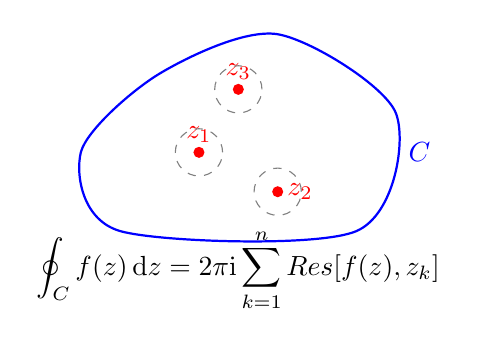
\begin{tikzpicture}[scale=1.0]
    \draw[blue, thick, ->] plot[smooth cycle] coordinates {(0,0) (3,0) (3.5,1.5) (2,2.5) (0.5,2) (-0.5,1)};
    \node[blue] at (3.8, 1) {$C$};

    \fill[red] (1, 1) circle (2pt) node[above] {$z_1$};
    \fill[red] (2, 0.5) circle (2pt) node[right] {$z_2$};
    \fill[red] (1.5, 1.8) circle (2pt) node[above] {$z_3$};

    \draw[gray, dashed] (1,1) circle (0.3);
    \draw[gray, dashed] (2,0.5) circle (0.3);
    \draw[gray, dashed] (1.5,1.8) circle (0.3);

    \node at (1.5,-0.5) {$\displaystyle \oint_C f(z)\,\mathrm{d}z = 2\pi \mathrm{i}\sum_{k=1}^n \operatorname{Res}[f(z),z_k]$};
\end{tikzpicture}
\caption{留数定理：整体闭路积分等于内部奇点的局部贡献之和}
\label{fig:residue-theorem}
\end{figure}

\begin{proof}
以每个奇点 $z_k$ 为圆心作一个足够小的圆 $C_k$，使这些小圆彼此互不相交，且都包含在 $D$ 内。把这些小圆盘从区域 $D$ 中挖去，得到一个多连通区域。由于所有奇点都已经被挖掉，所以 $f$ 在这个多连通区域内解析。

由多连通区域上的柯西积分定理，
\[
    \oint_C f(z)\,\mathrm{d}z
    =
    \sum_{k=1}^{n}\oint_{C_k} f(z)\,\mathrm{d}z.
\]
这里每个 $C_k$ 都取与外边界相适应的方向，故右边是各小围道积分之和。

又因为每个 $C_k$ 都只包围奇点 $z_k$，由上一节的小圆积分公式，
\[
    \oint_{C_k} f(z)\,\mathrm{d}z
    =
    2\pi \mathrm{i}\,\operatorname{Res}[f(z),z_k].
\]
把这些式子相加，就得到
\[
    \oint_C f(z)\,\mathrm{d}z
    =
    2\pi \mathrm{i}\sum_{k=1}^{n}\operatorname{Res}[f(z),z_k].
\]
\end{proof}

\begin{tishi}[留数定理真正重要在哪里]
留数定理把一个看起来属于\textbf{边界积分}的问题，转化成了若干个\textbf{局部系数}的代数求和问题。这就是它最核心的威力。以后你会越来越强烈地感受到：在复分析里，奇点附近的局部结构常常足以决定整体行为。
\end{tishi}

\subsection{留数定理的应用}

\begin{lizi}{多个奇点的闭路积分}{}
计算
\[
    \oint_{|z|=2}\frac{z+1}{z^2-1}\,\mathrm{d}z.
\]

\begin{jie}
先看奇点。由于
\[
    \frac{z+1}{z^2-1}
    =
    \frac{z+1}{(z-1)(z+1)},
\]
其中 $z=1$ 是真正的极点，而 $z=-1$ 处分子分母同为零，它其实是一个可去奇点。也就是说，延拓以后函数只在 $z=1$ 有一个简单极点。

因此围道 $|z|=2$ 内真正需要考虑的只有 $z=1$。

在 $z=1$ 处，
\[
    \operatorname{Res}\left[\frac{z+1}{z^2-1},1\right]
    =
    \lim_{z\to 1}(z-1)\frac{z+1}{(z-1)(z+1)}
    =1.
\]
于是由留数定理，
\[
    \oint_{|z|=2}\frac{z+1}{z^2-1}\,\mathrm{d}z
    =
    2\pi \mathrm{i}\cdot 1
    =
    2\pi \mathrm{i}.
\]
\end{jie}
\end{lizi}

\begin{lizi}{围道内外奇点的区别}{}
计算
\[
    \oint_{|z|=1}\frac{\mathrm{e}^z}{z(z-2)}\,\mathrm{d}z.
\]

\begin{jie}
函数的奇点为 $z=0$ 与 $z=2$。其中 $z=0$ 在圆 $|z|=1$ 内，而 $z=2$ 在圆外。

因此只需计算 $z=0$ 处的留数：
\[
    \operatorname{Res}\left[\frac{\mathrm{e}^z}{z(z-2)},0\right]
    =
    \lim_{z\to 0}
    z\cdot \frac{\mathrm{e}^z}{z(z-2)}
    =
    \lim_{z\to 0}\frac{\mathrm{e}^z}{z-2}
    =
    -\frac{1}{2}.
\]
于是
\[
    \oint_{|z|=1}\frac{\mathrm{e}^z}{z(z-2)}\,\mathrm{d}z
    =
    2\pi \mathrm{i}\cdot \left(-\frac{1}{2}\right)
    =
    -\pi \mathrm{i}.
\]
\end{jie}
\end{lizi}

\begin{jinshi}[一个必须先检查的条件]
使用留数定理前，首先要确认：\textbf{围道上不能有奇点。}如果奇点正好落在围道上，那么围道积分本身就需要重新解释，不能直接把留数定理硬套上去。
\end{jinshi}

\section{留数法计算积分的一般步骤}

\begin{wulibj}[本节的任务]
很多同学真正卡住的地方，不是在定理本身，而是在题目前：拿到一道积分题后，不知道该先找奇点、先选围道，还是先换元。本节不追求新公式，而是把留数法做题时最常见的判断流程整理出来。
\end{wulibj}

\begin{figure}[htbp]
\centering
\begin{tikzpicture}[
    node distance=0.75cm and 1.0cm,
    box/.style={rectangle, rounded corners=4pt, draw=blue!60!black, fill=blue!6, text width=3.1cm, minimum height=0.9cm, align=center, font=\small},
    arrow/.style={-{Stealth[length=2.3mm]}, thick, gray!75!black}
]
\node[box] (a) {先判断题型\\闭路积分、单位圆积分、无穷积分、振荡积分};
\node[box, below=of a] (b) {再找奇点\\位置、阶数、哪些在围道内};
\node[box, below=of b] (c) {再选围道\\单位圆、上半圆、下半圆或其他路径};
\node[box, below=of c] (d) {再算留数\\优先选最省力的方法};
\node[box, below=of d] (e) {再检查附加弧\\不能默认一定趋于零};
\node[box, below=of e] (f) {最后回到原积分\\注意实部、虚部、系数和方向};

\draw[arrow] (a) -- (b);
\draw[arrow] (b) -- (c);
\draw[arrow] (c) -- (d);
\draw[arrow] (d) -- (e);
\draw[arrow] (e) -- (f);
\end{tikzpicture}
\caption{留数法处理积分时的常见步骤}
\label{fig:residue-workflow}
\end{figure}

\subsection{先判断题目属于哪一类}

并不是所有积分题都要走同一条路线。通常至少要先分清下面几类：

\begin{enumerate}
    \item \textbf{闭路积分：}围道已经给定，此时重点是找出围道内部的奇点。
    \item \textbf{三角积分：}常见形状是
    \[
        \int_0^{2\pi} R(\cos\theta,\sin\theta)\,\mathrm{d}\theta,
    \]
    通常应想到单位圆代换 $z=\mathrm{e}^{\mathrm{i}\theta}$。
    \item \textbf{实轴无穷积分：}常见形状是
    \[
        \int_{-\infty}^{+\infty} R(x)\,\mathrm{d}x,
    \]
    常和大半圆围道有关。
    \item \textbf{带振荡因子的无穷积分：}例如
    \[
        \int_{-\infty}^{+\infty} R(x)\mathrm{e}^{\mathrm{i}ax}\,\mathrm{d}x,
    \]
    这时通常还要结合约当引理。
\end{enumerate}

\subsection{怎样找奇点与选围道}

题型判断清楚以后，下一步是找奇点，并思考它们与围道的位置关系。这里最容易忽略的是：\textbf{围道不是随便画的，它必须服务于原积分。}

\begin{itemize}
    \item 单位圆方法的围道不是猜出来的，而是由 $z=\mathrm{e}^{\mathrm{i}\theta}$ 这个换元自然给出的。
    \item 实轴无穷积分里常取上半圆或下半圆，但究竟选哪一侧，要看被积函数在那一侧是否更容易让附加弧积分消失。
    \item 若积分里出现 $\mathrm{e}^{\mathrm{i}ax}$，则上半平面还是下半平面的选择，通常由 $a$ 的符号决定。
\end{itemize}

\subsection{怎样检查附加路径积分}

留数法最容易被机械化的地方就在这里。很多人一看到半圆围道就默认``大圆弧积分一定趋于零''，这是很危险的。更稳妥的想法是：\textbf{先写估计，再判断是否真的趋于零。}

例如，对有理函数
\[
    R(z)=\frac{P(z)}{Q(z)},
\]
若分母次数比分子次数至少高 $2$，那么在大圆弧上往往有足够衰减；而若只高 $1$，就要更仔细地看。对含 $\mathrm{e}^{\mathrm{i}az}$ 的情形，则应额外利用指数因子在某个半平面的衰减。

\subsection{怎样把闭路积分还原成原积分}

复积分算完以后，还要回到原题。常见的回收方式有：

\begin{enumerate}
    \item \textbf{取实部或虚部：}很多 $\cos ax$、$\sin ax$ 型积分都要先转成 $\mathrm{e}^{\mathrm{i}ax}$，最后再取实部或虚部。
    \item \textbf{利用偶函数或奇函数：}例如
    \[
        \int_0^{+\infty}\frac{\cos x}{x^2+1}\,\mathrm{d}x
    \]
    常先补成整个实轴，再利用偶性除以 $2$。
    \item \textbf{注意换元带来的系数：}单位圆方法里
    \[
        \mathrm{d}\theta=\frac{\mathrm{d}z}{\mathrm{i}z},
    \]
    这个因子最容易漏。
\end{enumerate}

\begin{tishi}[把做题流程说成人话]
看到一道新题时，可以先问自己六个问题：
\begin{enumerate}
    \item 这是什么类型的积分？
    \item 它对应的复函数是什么？
    \item 奇点在哪里？
    \item 围道应该怎么选？
    \item 附加弧积分会不会消失？
    \item 最后该怎样回到原来的实积分？
\end{enumerate}
如果这六问都答得顺，留数法的思路一般就不会乱。
\end{tishi}

\begin{jinshi}[这一节最值得防的错误]
\begin{enumerate}
    \item 不要把``选围道''理解成背模板；围道必须和原积分结构匹配。
    \item 不要忘记检查附加弧积分。
    \item 不要在复积分算完后忘了回到原积分，尤其是取实部、取虚部和除以 $2$ 这几步。
\end{enumerate}
\end{jinshi}

\section{留数在实积分中的典型应用}

\begin{wulibj}[本节的任务]
前几节已经把工具准备好了。本节要真正展示留数理论的计算威力。为了让思路尽量顺畅，我们按难度递进来讲：先是单位圆方法处理三角积分，再是半圆围道处理有理型无穷积分，最后才是带振荡因子的积分与约当引理。
\end{wulibj}

\subsection{三角积分与单位圆方法}

考虑形如
\[
    \int_0^{2\pi} R(\cos\theta,\sin\theta)\,\mathrm{d}\theta
\]
的积分，其中 $R$ 是有理函数。最自然的换元是
\[
    z=\mathrm{e}^{\mathrm{i}\theta}.
\]
这样当 $\theta$ 从 $0$ 变到 $2\pi$ 时，$z$ 恰好沿单位圆逆时针走一周，并且
\[
    \cos\theta=\frac{z+z^{-1}}{2},\qquad
    \sin\theta=\frac{z-z^{-1}}{2\mathrm{i}},\qquad
    \mathrm{d}\theta=\frac{\mathrm{d}z}{\mathrm{i}z}.
\]

\begin{figure}[htbp]
\centering
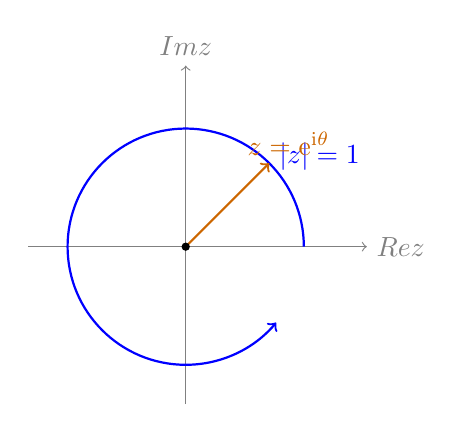
\begin{tikzpicture}[scale=1.0]
    \draw[->, gray] (-2,0) -- (2.3,0) node[right] {$\operatorname{Re} z$};
    \draw[->, gray] (0,-2) -- (0,2.3) node[above] {$\operatorname{Im} z$};
    \draw[blue, thick, ->] (1.5,0) arc[start angle=0,end angle=320,radius=1.5];
    \node[blue] at (1.7,1.15) {$|z|=1$};
    \draw[orange!80!black, thick, ->] (0,0) -- (45:1.5);
    \node[orange!80!black] at (45:1.85) {$z=\mathrm{e}^{\mathrm{i}\theta}$};
    \fill (0,0) circle (1.5pt);
\end{tikzpicture}
\caption{单位圆方法：$\theta$ 的积分转化为 $|z|=1$ 上的围道积分}
\label{fig:unit-circle-substitution}
\end{figure}

\begin{lizi}{单位圆方法的标准例题}{}
计算
\[
    I=\int_0^{2\pi}\frac{1}{1+a\cos\theta}\,\mathrm{d}\theta,
    \qquad 0<a<1.
\]

\begin{jie}
令 $z=\mathrm{e}^{\mathrm{i}\theta}$，则
\[
    \cos\theta=\frac{z+z^{-1}}{2},\qquad
    \mathrm{d}\theta=\frac{\mathrm{d}z}{\mathrm{i}z}.
\]
因此
\begin{align*}
    I
    &=
    \oint_{|z|=1}
    \frac{1}{1+\frac{a}{2}(z+z^{-1})}
    \cdot
    \frac{\mathrm{d}z}{\mathrm{i}z} \\
    &=
    \oint_{|z|=1}
    \frac{2\,\mathrm{d}z}{\mathrm{i}(az^2+2z+a)} \\
    &=
    \frac{2}{\mathrm{i}a}
    \oint_{|z|=1}
    \frac{\mathrm{d}z}{z^2+\frac{2}{a}z+1}.
\end{align*}

设
\[
    z^2+\frac{2}{a}z+1=0
\]
的两个根为 $z_1,z_2$。因为
\[
    z_1 z_2=1,
\]
所以这两个根中恰有一个在单位圆内。又由求根公式，
\[
    z_1-z_2=\frac{2\sqrt{1-a^2}}{a}.
\]
设 $z_1$ 为单位圆内的根，则被积函数在单位圆内只有一个简单极点 $z_1$，其留数为
\[
    \operatorname{Res}\left[\frac{1}{(z-z_1)(z-z_2)},z_1\right]
    =
    \frac{1}{z_1-z_2}.
\]
于是
\[
    I
    =
    \frac{2}{\mathrm{i}a}\cdot 2\pi \mathrm{i}\cdot \frac{1}{z_1-z_2}
    =
    \frac{4\pi}{a(z_1-z_2)}
    =
    \frac{2\pi}{\sqrt{1-a^2}}.
\]
\end{jie}
\end{lizi}

\begin{tishi}[单位圆方法的本质]
这类题的关键，并不只是记住
\[
    z=\mathrm{e}^{\mathrm{i}\theta}
\]
这个换元，而是意识到：它把三角函数问题改写成了\textbf{单位圆上的有理函数围道积分}。一旦改写完成，后面就是留数定理在工作。
\end{tishi}

\subsection{有理型无穷积分}

现在来看形如
\[
    \int_{-\infty}^{+\infty} R(x)\,\mathrm{d}x
\]
的积分，其中 $R$ 是有理函数。若分母次数比分子次数高得足够多，常见做法是在上半平面或下半平面补上一段大半圆，把实轴积分变成闭路积分。

\begin{figure}[htbp]
\centering
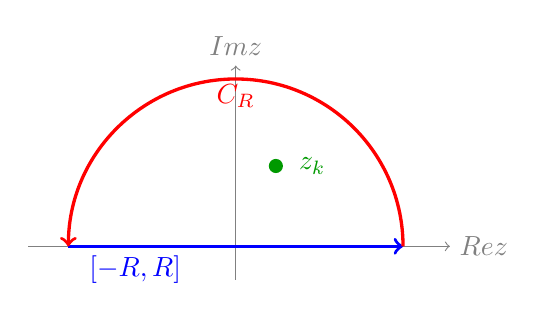
\begin{tikzpicture}[scale=0.85]
    \draw[->, gray] (-3.1,0) -- (3.2,0) node[right] {$\operatorname{Re} z$};
    \draw[->, gray] (0,-0.5) -- (0,2.7) node[above] {$\operatorname{Im} z$};

    \draw[blue, very thick, ->] (-2.5,0) -- (2.5,0);
    \draw[red, very thick, ->] (2.5,0) arc (0:180:2.5);
    \fill[green!60!black] (0.6,1.2) circle (3pt);
    \node[green!60!black, right] at (0.8,1.2) {$z_k$};
    \node[red] at (0,2.25) {$C_R$};
    \node[blue, below] at (-1.5,0) {$[-R,R]$};
\end{tikzpicture}
\caption{有理型无穷积分常用的上半平面围道}
\label{fig:upper-half-contour}
\end{figure}

\begin{lizi}{最标准的无穷积分}{}
计算
\[
    I=\int_{-\infty}^{+\infty}\frac{1}{x^2+a^2}\,\mathrm{d}x,
    \qquad a>0.
\]

\begin{jie}
取复函数
\[
    f(z)=\frac{1}{z^2+a^2}.
\]
它的极点是
\[
    z=\pm a\mathrm{i}.
\]
若取上半平面的半圆围道，则围道内部只有一个简单极点 $z=a\mathrm{i}$。

先计算该点的留数：
\[
    \operatorname{Res}[f(z),a\mathrm{i}]
    =
    \lim_{z\to a\mathrm{i}}
    \frac{z-a\mathrm{i}}{z^2+a^2}
    =
    \lim_{z\to a\mathrm{i}}
    \frac{1}{z+a\mathrm{i}}
    =
    \frac{1}{2a\mathrm{i}}.
\]

再看大半圆上的积分。设大半圆半径为 $R$，当 $R>a$ 时，在弧上有
\[
    |z^2+a^2|\ge |z|^2-a^2=R^2-a^2,
\]
因此
\[
    \left|\int_{C_R}\frac{1}{z^2+a^2}\,\mathrm{d}z\right|
    \le
    \frac{\pi R}{R^2-a^2}\to 0
    \qquad (R\to\infty).
\]
于是由留数定理，
\[
    I
    =
    2\pi \mathrm{i}\cdot \frac{1}{2a\mathrm{i}}
    =
    \frac{\pi}{a}.
\]
\end{jie}
\end{lizi}

\begin{lizi}{稍复杂的有理型无穷积分}{}
计算
\[
    I=\int_{-\infty}^{+\infty}\frac{x^2}{x^4+1}\,\mathrm{d}x.
\]

\begin{jie}
考虑
\[
    f(z)=\frac{z^2}{z^4+1}.
\]
方程
\[
    z^4+1=0
\]
的四个根是
\[
    \mathrm{e}^{\mathrm{i}\pi/4},\quad
    \mathrm{e}^{3\mathrm{i}\pi/4},\quad
    \mathrm{e}^{5\mathrm{i}\pi/4},\quad
    \mathrm{e}^{7\mathrm{i}\pi/4}.
\]
上半平面内的两个极点为
\[
    z_1=\mathrm{e}^{\mathrm{i}\pi/4},\qquad
    z_2=\mathrm{e}^{3\mathrm{i}\pi/4}.
\]

由于它们都是简单极点，而
\[
    (z^4+1)'=4z^3,
\]
所以
\[
    \operatorname{Res}[f(z),z_k]
    =
    \frac{z_k^2}{4z_k^3}
    =
    \frac{1}{4z_k}
    \qquad (k=1,2).
\]
因此
\[
    \operatorname{Res}[f(z),z_1]+\operatorname{Res}[f(z),z_2]
    =
    \frac{1}{4}\left(\frac{1}{z_1}+\frac{1}{z_2}\right).
\]
而
\[
    \frac{1}{z_1}=\mathrm{e}^{-\mathrm{i}\pi/4},\qquad
    \frac{1}{z_2}=\mathrm{e}^{-3\mathrm{i}\pi/4},
\]
故
\[
    \frac{1}{z_1}+\frac{1}{z_2}
    =
    \frac{1-\mathrm{i}}{\sqrt{2}}+\frac{-1-\mathrm{i}}{\sqrt{2}}
    =
    -\sqrt{2}\,\mathrm{i}.
\]
于是留数和为
\[
    -\frac{\mathrm{i}}{2\sqrt{2}}.
\]

再看大半圆上的积分。因为分母次数比分子次数高 $2$，与上一题同理，大圆弧上的积分趋于零。于是
\[
    I
    =
    2\pi \mathrm{i}\left(-\frac{\mathrm{i}}{2\sqrt{2}}\right)
    =
    \frac{\pi}{\sqrt{2}}.
\]
\end{jie}
\end{lizi}

\subsection{含振荡因子的无穷积分与约当引理}

当积分里出现
\[
    \mathrm{e}^{\mathrm{i}ax}
\]
这类振荡因子时，情况会比单纯的有理函数稍复杂一些。这里最核心的问题是：\textbf{大半圆弧上的积分为什么还能消失？}回答这个问题的常用工具就是约当引理。

\begin{dingli}{约当引理}{}
设 $f$ 在上半平面的充分大半圆及其内部除有限个点外解析，并且在半圆弧
\[
    C_R=\{z=R\mathrm{e}^{\mathrm{i}\theta}:0\le \theta\le \pi\}
\]
上满足
\[
    \max_{z\in C_R}|f(z)|\to 0
    \qquad (R\to\infty).
\]
则对任意 $a>0$，
\[
    \lim_{R\to\infty}\int_{C_R} f(z)\mathrm{e}^{\mathrm{i}az}\,\mathrm{d}z=0.
\]
\end{dingli}

\begin{figure}[htbp]
\centering
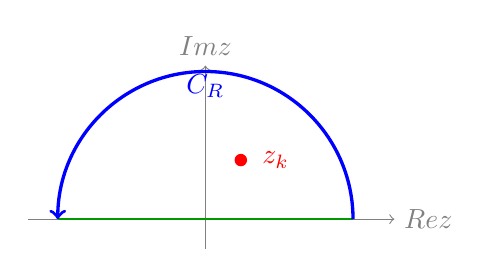
\begin{tikzpicture}[scale=0.75]
    \draw[->, gray] (-3.0,0) -- (3.2,0) node[right] {$\operatorname{Re} z$};
    \draw[->, gray] (0,-0.5) -- (0,2.6) node[above] {$\operatorname{Im} z$};

    \draw[green!60!black, thick] (-2.5,0) -- (2.5,0);
    \draw[blue, very thick, ->] (2.5,0) arc (0:180:2.5);
    \fill[red] (0.6,1.0) circle (3pt);
    \node[red, right] at (0.8,1.0) {$z_k$};
    \node[blue] at (0,2.25) {$C_R$};
\end{tikzpicture}
\caption{含 $\mathrm{e}^{\mathrm{i}az}$ 的积分常用围道}
\label{fig:jordan-contour-ch05}
\end{figure}

\begin{proof}
设
\[
    M_R=\max_{z\in C_R}|f(z)|.
\]
在半圆弧上令 $z=R\mathrm{e}^{\mathrm{i}\theta}$，则
\[
    \mathrm{d}z=\mathrm{i}R\mathrm{e}^{\mathrm{i}\theta}\,\mathrm{d}\theta,
    \qquad 0\le \theta\le \pi.
\]
又因为
\[
    \left|\mathrm{e}^{\mathrm{i}az}\right|
    =
    \left|\mathrm{e}^{\mathrm{i}aR(\cos\theta+\mathrm{i}\sin\theta)}\right|
    =
    \mathrm{e}^{-aR\sin\theta},
\]
所以
\[
    \left|\int_{C_R} f(z)\mathrm{e}^{\mathrm{i}az}\,\mathrm{d}z\right|
    \le
    M_R R\int_0^\pi \mathrm{e}^{-aR\sin\theta}\,\mathrm{d}\theta.
\]
而标准估计给出
\[
    \int_0^\pi \mathrm{e}^{-aR\sin\theta}\,\mathrm{d}\theta
    \le
    \frac{\pi}{aR}.
\]
于是
\[
    \left|\int_{C_R} f(z)\mathrm{e}^{\mathrm{i}az}\,\mathrm{d}z\right|
    \le
    \frac{\pi M_R}{a}\to 0.
\]
故结论成立。
\end{proof}

\begin{lizi}{由复指数转回余弦积分}{}
计算
\[
    I=\int_0^{+\infty}\frac{\cos x}{x^2+1}\,\mathrm{d}x.
\]

\begin{jie}
先考虑整个实轴上的复积分
\[
    J=\int_{-\infty}^{+\infty}\frac{\mathrm{e}^{\mathrm{i}x}}{x^2+1}\,\mathrm{d}x.
\]
取复函数
\[
    f(z)=\frac{\mathrm{e}^{\mathrm{i}z}}{z^2+1},
\]
并在上半平面闭合围道。因为 $a=1>0$，指数因子在上半平面有衰减，所以可用约当引理说明大圆弧上的积分趋于零。

围道内部只有一个简单极点 $z=\mathrm{i}$。其留数为
\[
    \operatorname{Res}[f(z),\mathrm{i}]
    =
    \lim_{z\to \mathrm{i}}
    \frac{(z-\mathrm{i})\mathrm{e}^{\mathrm{i}z}}{(z-\mathrm{i})(z+\mathrm{i})}
    =
    \frac{\mathrm{e}^{\mathrm{i}\cdot \mathrm{i}}}{2\mathrm{i}}
    =
    \frac{\mathrm{e}^{-1}}{2\mathrm{i}}.
\]
因此
\[
    J
    =
    2\pi \mathrm{i}\cdot \frac{\mathrm{e}^{-1}}{2\mathrm{i}}
    =
    \frac{\pi}{\mathrm{e}}.
\]

另一方面，
\[
    J
    =
    \int_{-\infty}^{+\infty}\frac{\cos x}{x^2+1}\,\mathrm{d}x
    +
    \mathrm{i}
    \int_{-\infty}^{+\infty}\frac{\sin x}{x^2+1}\,\mathrm{d}x.
\]
其中虚部对应的积分是奇函数在对称区间上的积分，因此为零，所以
\[
    \int_{-\infty}^{+\infty}\frac{\cos x}{x^2+1}\,\mathrm{d}x
    =
    \frac{\pi}{\mathrm{e}}.
\]
又因为被积函数是偶函数，于是
\[
    I
    =
    \frac{1}{2}\cdot \frac{\pi}{\mathrm{e}}
    =
    \frac{\pi}{2\mathrm{e}}.
\]
\end{jie}
\end{lizi}

\begin{lizi}{由复指数转回正弦积分}{}
计算
\[
    I=\int_0^{+\infty}\frac{x\sin x}{x^2+1}\,\mathrm{d}x.
\]

\begin{jie}
考虑
\[
    J=\int_{-\infty}^{+\infty}\frac{x\mathrm{e}^{\mathrm{i}x}}{x^2+1}\,\mathrm{d}x.
\]
取
\[
    f(z)=\frac{z\mathrm{e}^{\mathrm{i}z}}{z^2+1}.
\]
与上一题同理，取上半平面围道，大圆弧积分由约当引理趋于零。

围道内部仍只有极点 $z=\mathrm{i}$。其留数为
\[
    \operatorname{Res}[f(z),\mathrm{i}]
    =
    \lim_{z\to \mathrm{i}}
    \frac{z\mathrm{e}^{\mathrm{i}z}}{z+\mathrm{i}}
    =
    \frac{\mathrm{i}\mathrm{e}^{-1}}{2\mathrm{i}}
    =
    \frac{\mathrm{e}^{-1}}{2}.
\]
因此
\[
    J=2\pi \mathrm{i}\cdot \frac{\mathrm{e}^{-1}}{2}
    =
    \frac{\pi \mathrm{i}}{\mathrm{e}}.
\]

再把 $J$ 拆成实部和虚部：
\[
    J
    =
    \int_{-\infty}^{+\infty}\frac{x\cos x}{x^2+1}\,\mathrm{d}x
    +
    \mathrm{i}
    \int_{-\infty}^{+\infty}\frac{x\sin x}{x^2+1}\,\mathrm{d}x.
\]
其中第一项是奇函数在对称区间上的积分，因此为零。所以
\[
    \int_{-\infty}^{+\infty}\frac{x\sin x}{x^2+1}\,\mathrm{d}x
    =
    \frac{\pi}{\mathrm{e}}.
\]
而
\[
    \frac{x\sin x}{x^2+1}
\]
是偶函数，因此
\[
    I
    =
    \frac{1}{2}\cdot \frac{\pi}{\mathrm{e}}
    =
    \frac{\pi}{2\mathrm{e}}.
\]
\end{jie}
\end{lizi}

\section{对数留数、辐角原理与鲁歇定理（选读）}

\begin{wulibj}[本节的任务]
前面几节强调的是留数在\textbf{积分计算}中的作用；本节则想让学生进一步看到，留数还可以用来研究\textbf{零点和极点的个数}。关键对象是
\[
    \frac{f'(z)}{f(z)}.
\]
它会把零点和极点的重数直接转化为留数，于是``数根问题''也就可以转化为积分问题。
\end{wulibj}

\begin{tishi}[选读说明]
这一节在逻辑上和前面的主线是连着的，但学习重心已经从``算积分''转向``数零点''。如果课程重点更偏计算应用，可以把这一节作为选读；如果后面准备进一步讲映射理论，那么这一节就会成为非常重要的桥梁。
\end{tishi}

\subsection{\texorpdfstring{为什么考虑 $f'(z)/f(z)$}{为什么考虑 f'(z)/f(z)}}

如果我们想知道某个区域里有多少个零点和极点，最自然的想法是：找一个函数，它在零点和极点附近能把``重数''直接暴露出来。对数导数
\[
    \frac{f'(z)}{f(z)}
\]
恰好就有这种性质。

\begin{dingli}{\texorpdfstring{$f'(z)/f(z)$}{f'(z)/f(z)} 在零点与极点处的留数}{}
设 $z_0$ 是 $f$ 的孤立零点或孤立极点。
\begin{enumerate}
    \item 若 $z_0$ 是 $f$ 的 $m$ 阶零点，则
    \[
        \operatorname{Res}\left[\frac{f'(z)}{f(z)},z_0\right]=m.
    \]
    \item 若 $z_0$ 是 $f$ 的 $m$ 阶极点，则
    \[
        \operatorname{Res}\left[\frac{f'(z)}{f(z)},z_0\right]=-m.
    \]
\end{enumerate}
\end{dingli}

\begin{proof}
先设 $z_0$ 是 $f$ 的 $m$ 阶零点，则可写成
\[
    f(z)=(z-z_0)^m g(z),
\]
其中 $g$ 在 $z_0$ 附近解析且 $g(z_0)\neq 0$。对两边求导并除以 $f(z)$，得
\[
    \frac{f'(z)}{f(z)}
    =
    \frac{m}{z-z_0}+\frac{g'(z)}{g(z)}.
\]
第二项在 $z_0$ 附近解析，所以其留数为零。因此
\[
    \operatorname{Res}\left[\frac{f'(z)}{f(z)},z_0\right]=m.
\]

若 $z_0$ 是 $m$ 阶极点，则可写成
\[
    f(z)=\frac{g(z)}{(z-z_0)^m},
\]
其中 $g$ 在 $z_0$ 附近解析且 $g(z_0)\neq 0$。于是
\[
    \frac{f'(z)}{f(z)}
    =
    \frac{g'(z)}{g(z)}-\frac{m}{z-z_0},
\]
所以对应留数为 $-m$。
\end{proof}

\subsection{对数留数与辐角原理}

\begin{dingliyi}{对数留数}{}
设 $f$ 在简单闭曲线 $C$ 上不为零，并且在 $C$ 的内部只有有限个零点和极点，则
\[
    \frac{1}{2\pi \mathrm{i}}\oint_C \frac{f'(z)}{f(z)}\,\mathrm{d}z
\]
称为 $f$ 关于曲线 $C$ 的\textbf{对数留数}。
\end{dingliyi}

\begin{dingli}{辐角原理}{}
设 $f$ 在简单闭曲线 $C$ 上解析且不为零，在 $C$ 内部有 $N$ 个零点和 $P$ 个极点，均按重数计，则
\[
    \frac{1}{2\pi \mathrm{i}}
    \oint_C \frac{f'(z)}{f(z)}\,\mathrm{d}z
    =
    N-P.
\]
\end{dingli}

\begin{proof}
由上一条定理可知，函数
\[
    \frac{f'(z)}{f(z)}
\]
在 $f$ 的每个零点和极点处都有简单极点，而且留数分别是相应零点重数和极点重数的相反数。因此由留数定理，
\[
    \oint_C \frac{f'(z)}{f(z)}\,\mathrm{d}z
    =
    2\pi \mathrm{i}(N-P).
\]
两边再除以 $2\pi \mathrm{i}$，便得到结论。
\end{proof}

\begin{tishi}[辐角原理的几何意义]
当 $z$ 沿曲线 $C$ 走一周时，像点 $w=f(z)$ 也会在像平面中走出一条闭曲线。辐角原理说明：这条像曲线绕原点的圈数，正好等于 $C$ 内部零点总重数减去极点总重数。
\end{tishi}

\subsection{鲁歇定理}

\begin{dingli}{鲁歇定理}{}
设 $f$ 和 $g$ 在简单闭曲线 $C$ 上及其内部解析，并且在 $C$ 上满足
\[
    |f(z)|>|g(z)|,
\]
则 $f$ 与 $f+g$ 在 $C$ 内部有相同个数的零点，按重数计。
\end{dingli}

\begin{proof}
考虑一族函数
\[
    h_t(z)=f(z)+tg(z),\qquad 0\le t\le 1.
\]
在曲线 $C$ 上，由条件
\[
    |h_t(z)|
    \ge |f(z)|-t|g(z)|
    \ge |f(z)|-|g(z)|
    >0,
\]
所以对所有 $t\in[0,1]$，$h_t$ 在 $C$ 上都不为零。

于是由辐角原理，
\[
    N(t)=\frac{1}{2\pi \mathrm{i}}\oint_C \frac{h_t'(z)}{h_t(z)}\,\mathrm{d}z
\]
给出 $h_t$ 在 $C$ 内的零点个数。由于积分关于 $t$ 连续变化，而 $N(t)$ 只能取整数值，所以 $N(t)$ 必为常数。

当 $t=0$ 时，$h_t=f$；当 $t=1$ 时，$h_t=f+g$。因此二者在 $C$ 内部的零点个数相同。
\end{proof}

\begin{lizi}{用鲁歇定理数根}{}
证明方程
\[
    z^8-5z^5-2z+1=0
\]
在单位圆内有 $5$ 个根。

\begin{jie}
在单位圆 $|z|=1$ 上取
\[
    f(z)=-5z^5,\qquad g(z)=z^8-2z+1.
\]
则
\[
    |f(z)|=5,
\]
而
\[
    |g(z)|\le |z|^8+2|z|+1=1+2+1=4.
\]
因此在单位圆上有
\[
    |f(z)|>|g(z)|.
\]
由鲁歇定理，$f$ 与 $f+g=z^8-5z^5-2z+1$ 在单位圆内有相同数目的零点。

而
\[
    f(z)=-5z^5
\]
在单位圆内只有一个零点 $z=0$，但它是 $5$ 重零点，所以零点总数按重数计为 $5$。因此原方程在单位圆内有 $5$ 个根。
\end{jie}
\end{lizi}

\section{本章小结}

\begin{tishi}[一句话回看本章]
本章最核心的事情，是把奇点附近的局部展开进一步压缩成一个关键系数，并说明这个系数怎样控制闭路积分、实积分，乃至零点与极点的计数。换句话说，本章真正建立起来的，是``局部信息如何进入整体计算''的眼光。
\end{tishi}

\begin{figure}[htbp]
\centering
\begin{tikzpicture}[
    node distance=1.0cm and 1.8cm,
    concept/.style={rectangle, rounded corners=4pt, draw=blue!60!black, fill=blue!6, text width=3.3cm, minimum height=0.85cm, align=center, font=\small},
    result/.style={rectangle, rounded corners=4pt, draw=green!60!black, fill=green!8, text width=3.4cm, minimum height=0.85cm, align=center, font=\small},
    arrow/.style={-{Stealth[length=2.4mm]}, thick, gray!75!black}
]
\node[concept] (laurent) {洛朗展开\\负幂项记录奇点结构};
\node[result, below=of laurent] (res) {$c_{-1}$ 的特殊地位\\$\Longrightarrow$ 留数};
\node[concept, below left=1.2cm and 0.8cm of res] (thm) {留数定理\\局部系数控制整体积分};
\node[concept, below right=1.2cm and 0.8cm of res] (calc) {实积分应用\\单位圆方法、半圆围道、约当引理};
\node[result, below=1.2cm of res] (count) {$\dfrac{f'}{f}$ 的留数\\$\Longrightarrow$ 零点与极点计数};

\draw[arrow] (laurent) -- (res);
\draw[arrow] (res) -- (thm);
\draw[arrow] (res) -- (calc);
\draw[arrow] (thm) -- (count);
\draw[arrow] (calc) -- (count);
\end{tikzpicture}
\caption{本章知识主线：从局部系数走向整体积分与零点计数}
\label{fig:ch05-knowledge-map}
\end{figure}

\begin{zhongyao}[本章主要结论]
\raggedright
\begin{enumerate}
    \item \textbf{留数就是洛朗展开中的 $c_{-1}$：}它不是附加记号，而是被围道积分自动筛选出来的那一个特殊系数。
    \item \textbf{小圆积分只留下留数项：}若围绕孤立奇点作小圆积分，则
    \[
        \oint f(z)\,\mathrm{d}z = 2\pi \mathrm{i}\,\operatorname{Res}.
    \]
    这说明围道积分对局部展开有非常强的选择性。
    \item \textbf{留数定理把闭路积分化成局部贡献之和：}对有限个孤立奇点，整体闭路积分等于内部各点留数总和乘上 $2\pi \mathrm{i}$。
    \item \textbf{求留数时应先分类、再选法：}简单极点优先极限法或 $\dfrac{P(z_0)}{Q'(z_0)}$，高阶极点再考虑导数公式，容易展开的函数则可直接读洛朗展开。
    \item \textbf{留数法处理实积分时，围道选择是核心：}三角积分常转到单位圆上；有理型无穷积分常用大半圆围道；带振荡因子的积分则要结合约当引理。
    \item \textbf{$\dfrac{f'}{f}$ 的留数能读出零点与极点的重数：}这使留数理论自然延伸到辐角原理与鲁歇定理。
\end{enumerate}
\end{zhongyao}

\begin{tishi}[做题时的判断思路]
\begin{enumerate}
    \item 看到奇点问题，先问自己：要找的是奇点类型、主部，还是留数？
    \item 看到``求留数''，先判断该点是简单极点还是高阶极点，再决定是用极限法、快捷公式、导数公式，还是直接展开。
    \item 看到闭路积分，先数清围道内部到底有哪些奇点，不要把围道外的点也算进去。
    \item 看到三角积分，优先想到 $z=\mathrm{e}^{\mathrm{i}\theta}$。
    \item 看到实轴无穷积分，先问附加弧积分是否真的趋于零。
    \item 看到零点个数问题，则应想到 $\dfrac{f'}{f}$、辐角原理或鲁歇定理。
\end{enumerate}
\end{tishi}

\begin{jinshi}[本章最容易混淆的地方]
\begin{enumerate}
    \item 不要把留数看成奇点的全部信息；它只是主部里最特殊的那一项系数。
    \item 不要把``留数为零''误读成``该点解析''。
    \item 不要忘记留数定理要求围道上没有奇点。
    \item 不要做实积分时只顾求留数，而忘了检查附加弧积分和回收原积分。
    \item 不要在辐角原理和鲁歇定理里忘记``按重数计''这几个字。
\end{enumerate}
\end{jinshi}

\begin{tishi}[和前后内容的联系]
回头看，本章并不是凭空开始的。第四章最后通过洛朗展开说明了一阶负幂项的特殊地位，本章只是把这一观察正式提升为留数概念，并把它发展成留数定理。换句话说，本章的根扎在上一章的局部展开理论里。

往后看，本章的围道积分技巧会在傅里叶变换、拉普拉斯逆变换等内容中反复出现；而本章末尾的辐角原理和鲁歇定理，又会把学生带向更整体、更几何的复分析视角。所以留数理论恰好站在``局部展开''、``积分计算''和``零点分布''三条线的交汇处，是整段复变函数内容中承上启下的一章。
\end{tishi}

\section{习题}

\subsection*{基础题}

\begin{enumerate}
    \item 求下列函数在指定点处的留数：
    \begin{enumerate}
        \item $\displaystyle f(z)=\frac{z}{z^2+1},\quad z=\mathrm{i}$；
        \item $\displaystyle f(z)=\frac{1}{(z-1)^3},\quad z=1$；
        \item $\displaystyle f(z)=\frac{\mathrm{e}^z}{z(z-1)},\quad z=0,1$。
    \end{enumerate}

    \item 用留数定理计算：
    \begin{enumerate}
        \item $\displaystyle \oint_{|z|=2}\frac{z}{z^2-1}\,\mathrm{d}z$；
        \item $\displaystyle \oint_{|z|=1}\frac{\sin z}{z}\,\mathrm{d}z$。
    \end{enumerate}

    \item 判断下列说法是否正确，并说明理由：
    \begin{enumerate}
        \item 留数为零的点一定不是奇点；
        \item 围道内部奇点越多，闭路积分一定越大；
        \item 高阶极点的留数一定非零。
    \end{enumerate}
\end{enumerate}

\subsection*{综合题}

\begin{enumerate}
    \item 计算下列实积分：
    \begin{enumerate}
        \item $\displaystyle \int_0^{2\pi}\frac{1}{2+\cos\theta}\,\mathrm{d}\theta$；
        \item $\displaystyle \int_{-\infty}^{+\infty}\frac{x^2}{x^4+1}\,\mathrm{d}x$；
        \item $\displaystyle \int_0^{+\infty}\frac{x\sin x}{x^2+1}\,\mathrm{d}x$。
    \end{enumerate}

    \item 设
    \[
        f(z)=\frac{z^2+3z+1}{(z-1)^2(z+1)},
    \]
    求它在各个有限奇点处的留数，并计算
    \[
        \oint_{|z|=2} f(z)\,\mathrm{d}z.
    \]

    \item 用辐角原理说明：若 $f$ 在简单闭曲线 $C$ 上不为零，则
    \[
        \frac{1}{2\pi \mathrm{i}}\oint_C \frac{f'(z)}{f(z)}\,\mathrm{d}z
    \]
    一定是整数。
\end{enumerate}

\subsection*{挑战题}

\begin{enumerate}
    \item 证明：当 $a>|b|>0$ 时，
    \[
        \int_0^{2\pi}\frac{1}{a+b\cos\theta}\,\mathrm{d}\theta
        =
        \frac{2\pi}{\sqrt{a^2-b^2}}.
    \]

    \item 用鲁歇定理证明：方程
    \[
        z^5-z+1=0
    \]
    在单位圆内有 $1$ 个根。

    \item 设 $f$ 在简单闭曲线 $C$ 上及其内部解析，且在 $C$ 上满足
    \[
        |f(z)-z^n|<|z|^n.
    \]
    证明 $f$ 在 $C$ 内部有与 $z^n$ 相同数目的零点。
\end{enumerate}
